\section{Dataset} % todo: rename to dataset generation
\label{sec:training_of_the_cnn:dataset}
% \todo[inline]{too much 'the' in the very last section, layout, citations, todos, cleanup}

% todo: mention that this dataset is available as .tar.gz
% todo: mention the total size (~27 GB)
The dataset contains frames of 22 different throwing objects, as shown in table \ref{tab:objects}.
It is fully labeled and consists of more than \num{15000} usable frames with at least \num{485} frames of each object.
All frames were collected over the course of two days during the previous project.
% Figure \ref{subfig:dataset_stuffed_bunny} shows an example frame of the \textit{Stuffed Bunny} and figure \ref{subfig:dataset_hand_featherball} shows an frame of the \textit{Hand Featherball}.
% Figure \ref{fig:dataset} shows two example frames from the dataset, the \textit{Stuffed Bunny} and the \textit{Hand Featherball}.
Figure \ref{fig:dataset} shows two example frames from the dataset (the \textit{Stuffed Bunny} and the \textit{Hand Featherball}).

\begin{table}
  \caption{List of the different throwing objects}
  \label{tab:objects}
  \centering
  \begin{tabular}{llll}
    \toprule
    \textbf{Objects} &  &  &  \\
    \midrule
    Nerf Dart & American Football & Table Tennis Ball & Shuttlecock \\ % left to right, top to bottom
    Sporf & Arrow & Hand Featherball & Floorball \\
    Spiky Ball & Tesafilm & Sponge & Red Duplo Brick \\
    Green Duplo Brick & Duplo Figure & Foam Die & Infant Shoe \\
    Stuffed Bunny & Goalkeeper Glove & Hemp Cord & Paper Ball \\
    Beer Cap & Water Bottle &  &  \\
    \bottomrule
  \end{tabular}
\end{table}

\begin{figure}[t]
  \centering
  \begin{subfigure}[b]{0.45\textwidth}
    \centering
    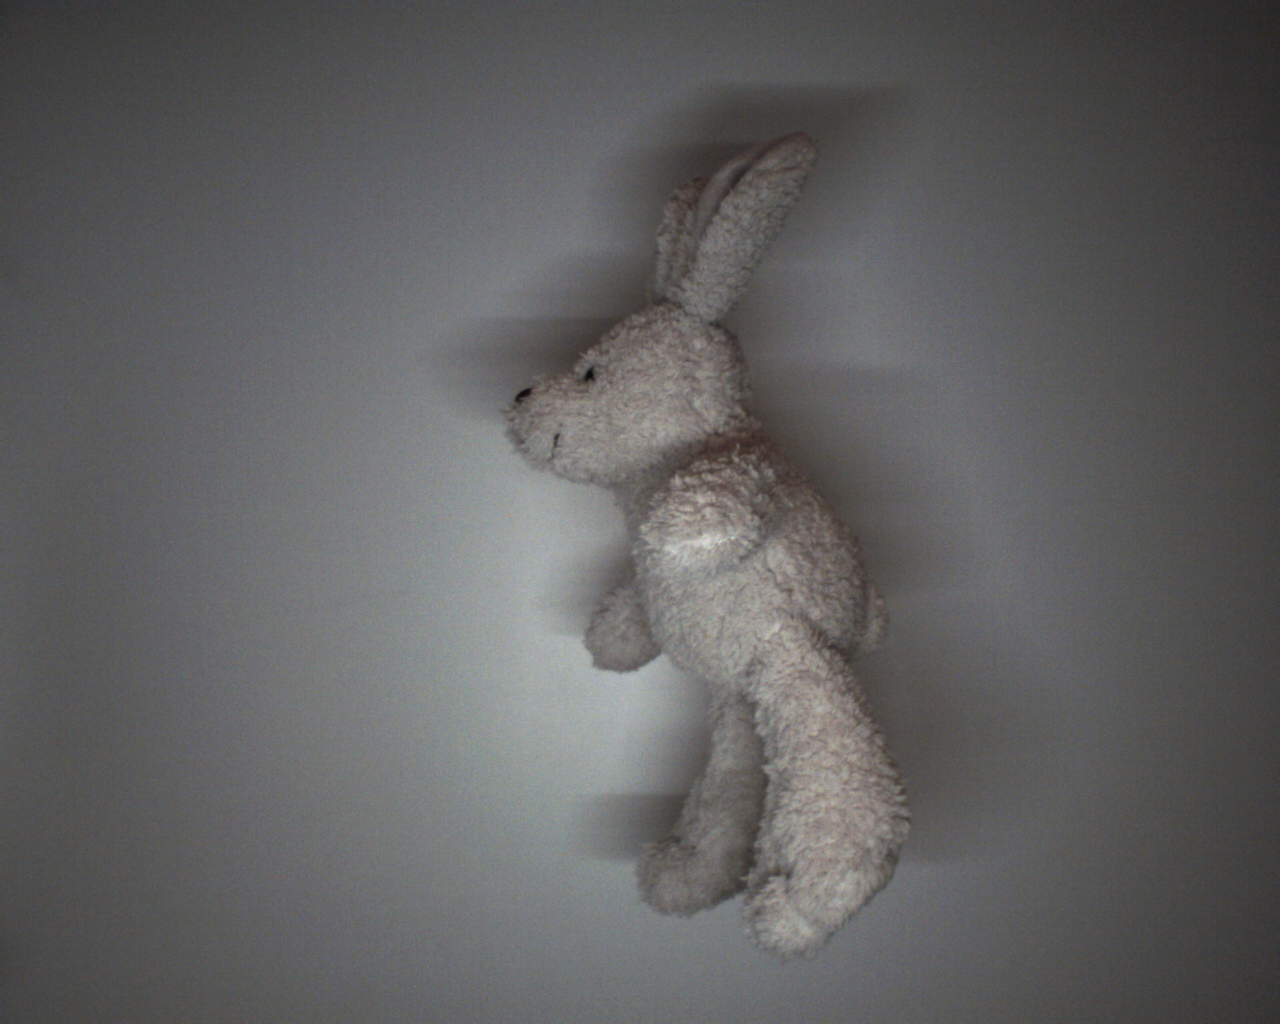
\includegraphics[width=\textwidth]{1574952009_278_10_stuffed-bunny}
    \caption{Stuffed Bunny}
    \label{subfig:dataset_stuffed_bunny}
  \end{subfigure}
  \begin{subfigure}[b]{0.45\textwidth}
    \centering
    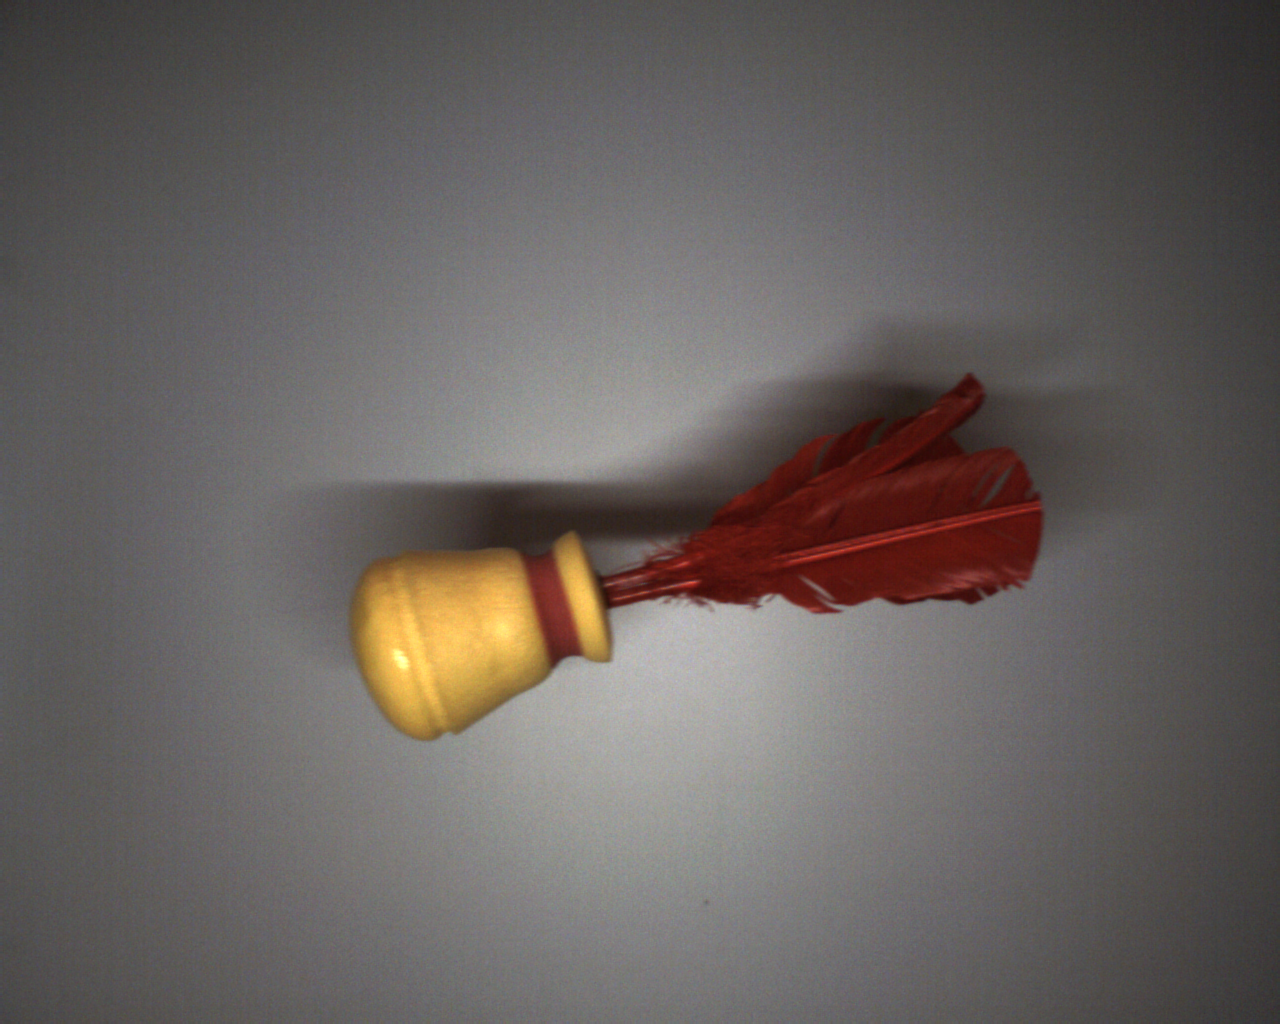
\includegraphics[width=\textwidth]{1574943825_125_8_hand-featherball}
    \caption{Hand Featherball}
    \label{subfig:dataset_hand_featherball}
  \end{subfigure}
  \caption{Two example frames from the dataset}
  \label{fig:dataset}
\end{figure}





\subsection{White Balance}
\label{subsec:training_of_the_cnn:dataset:white_balance}

A notable thing is that on the first day of the data collection, the white balance was performed continuously (every three frames). % todo: frame or data collection?
This caused the background color of large colored objects to be distorted, as shown in figure \ref{fig:white_balance}.
However, this is not problematic, as noise can improve the generalization and thus reduce overfitting \cite{}. % todo: cite https://machinelearningmastery.com/train-neural-networks-with-noise-to-reduce-overfitting/

\begin{figure}[t]
  \centering
  \begin{subfigure}[b]{0.45\textwidth}
    \centering
    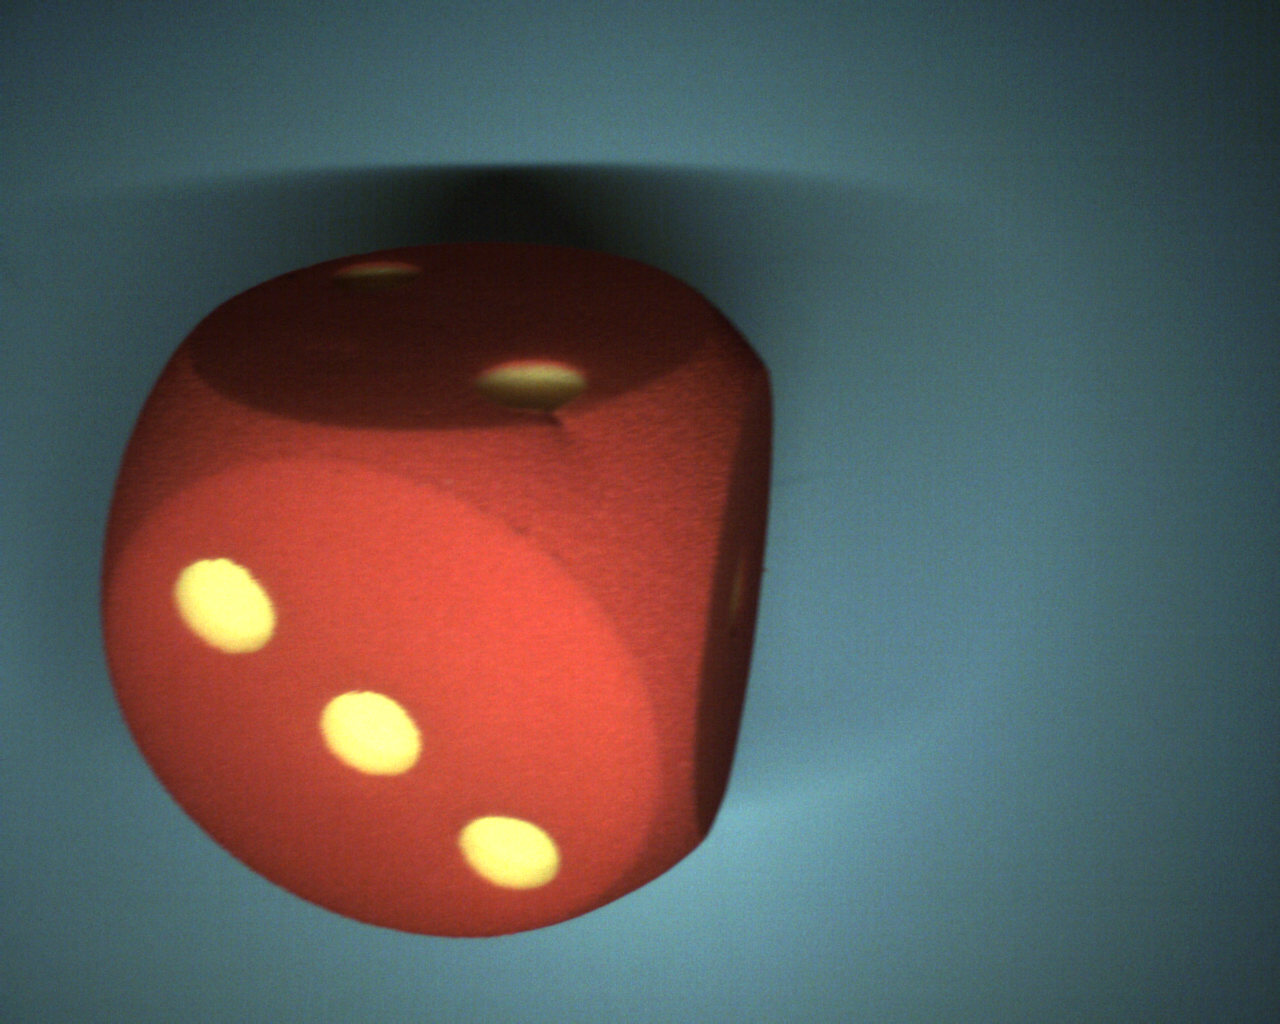
\includegraphics[width=\textwidth]{1574950250_238_9_foam-dice} % todo: was 0.9\textwidth better?
    \caption{Continuous white balance}
    \label{subfig:white_balance_first_day}
  \end{subfigure}
  \begin{subfigure}[b]{0.45\textwidth}
    \centering
    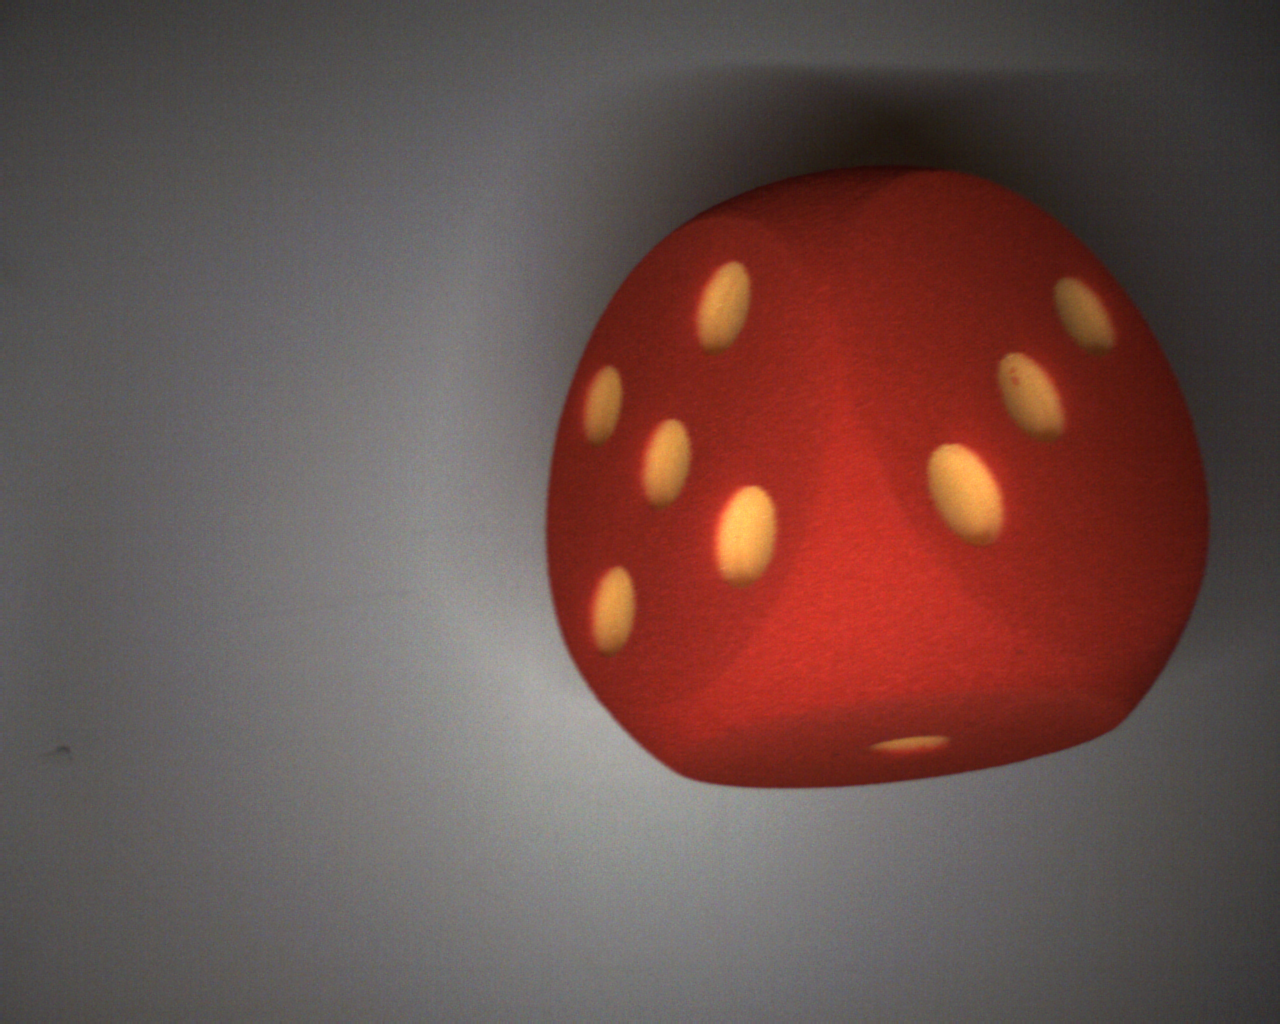
\includegraphics[width=\textwidth]{1575032343_726_8_foam-dice}
    \caption{One-off white balance}
    \label{subfig:white_balance_second_day}
  \end{subfigure}
  \caption{White balance difference between the first (\subref{subfig:white_balance_first_day}) and the second (\subref{subfig:white_balance_second_day}) day}
  \label{fig:white_balance}
\end{figure}








\subsection{Statistics}
\label{subsec:training_of_the_cnn:dataset:statistics}

Figure \ref{fig:statistics} shows the amount of captured frames for each object individually.
It is evident that there are generally more frames of larger objects.
This is, on the one hand, due to the specific implementation of the throw detection mechanism (see section \ref{}). % todo: reference to the description of the throw detection mechanism
On the other hand, the field of view of the camera is not uniformly illuminated (the center is brighter than the edges).
For those reasons, a larger object area is required at the borders to achieve a sufficiently large change in the frame.
However, this also leads to the fact that larger objects are more often only partially in the frame.

% Class imbalance problem
% This is an example of a slightly imbalanced dataset
The statistics of the dataset reveal that it is slightly imbalanced.
% An important aspect of the dataset is
% has to be taken into account when creating the splits (see section xyz)
This fact has to be taken into account when creating the various dataset splits (see section \ref{subsec:training_of_the_cnn:dataset:splitting}) that are required for the fitting and evaluation of the model.

% An imbalanced dataset can lead to serious problems, such as to a bias towards the classes with the most samples.
An imbalanced dataset can lead to serious problems, e.g. a bias towards the classes with the most samples.
% An imbalanced dataset can lead to a bias towards the classes with the most samples.
% If, for example, a dataset consisting of two classes is imbalanced in such a way that \SI{90}{\percent} of all samples belong to class \texttt{A}
Consider a dataset consisting of only two classes that is imbalanced in such a way that \SI{90}{\percent} of all samples belong to class \texttt{A}.
The fitting process of the classification model will naturally favor class \texttt{A}, since the chance of being right is nine times higher.
% Classifying every input to class \texttt{A} would result in a \SI{90}{\percent} accuracy.
% During the fitting of the classification model it could
% no matter the input will result in class \texttt{A}
% The classification could then be independent of the input and always opt for class \texttt{A} (completely ignoring class \texttt{B}). % not good due to the previous sentence
The classification could even be independent of the input and always opt for class \texttt{A} (completely ignoring class \texttt{B}).
This obviously terrible classification process would still result in an overall accuracy of \SI{90}{\percent} \cite{}. % todo: cite https://machinelearningmastery.com/tactics-to-combat-imbalanced-classes-in-your-machine-learning-dataset/

% http://www.chioka.in/class-imbalance-problem/ (bad source)
% https://machinelearningmastery.com/what-is-imbalanced-classification/ (A Gentle Introduction to Imbalanced Classification, prob. not what I want)

\begin{figure}
  \centering
  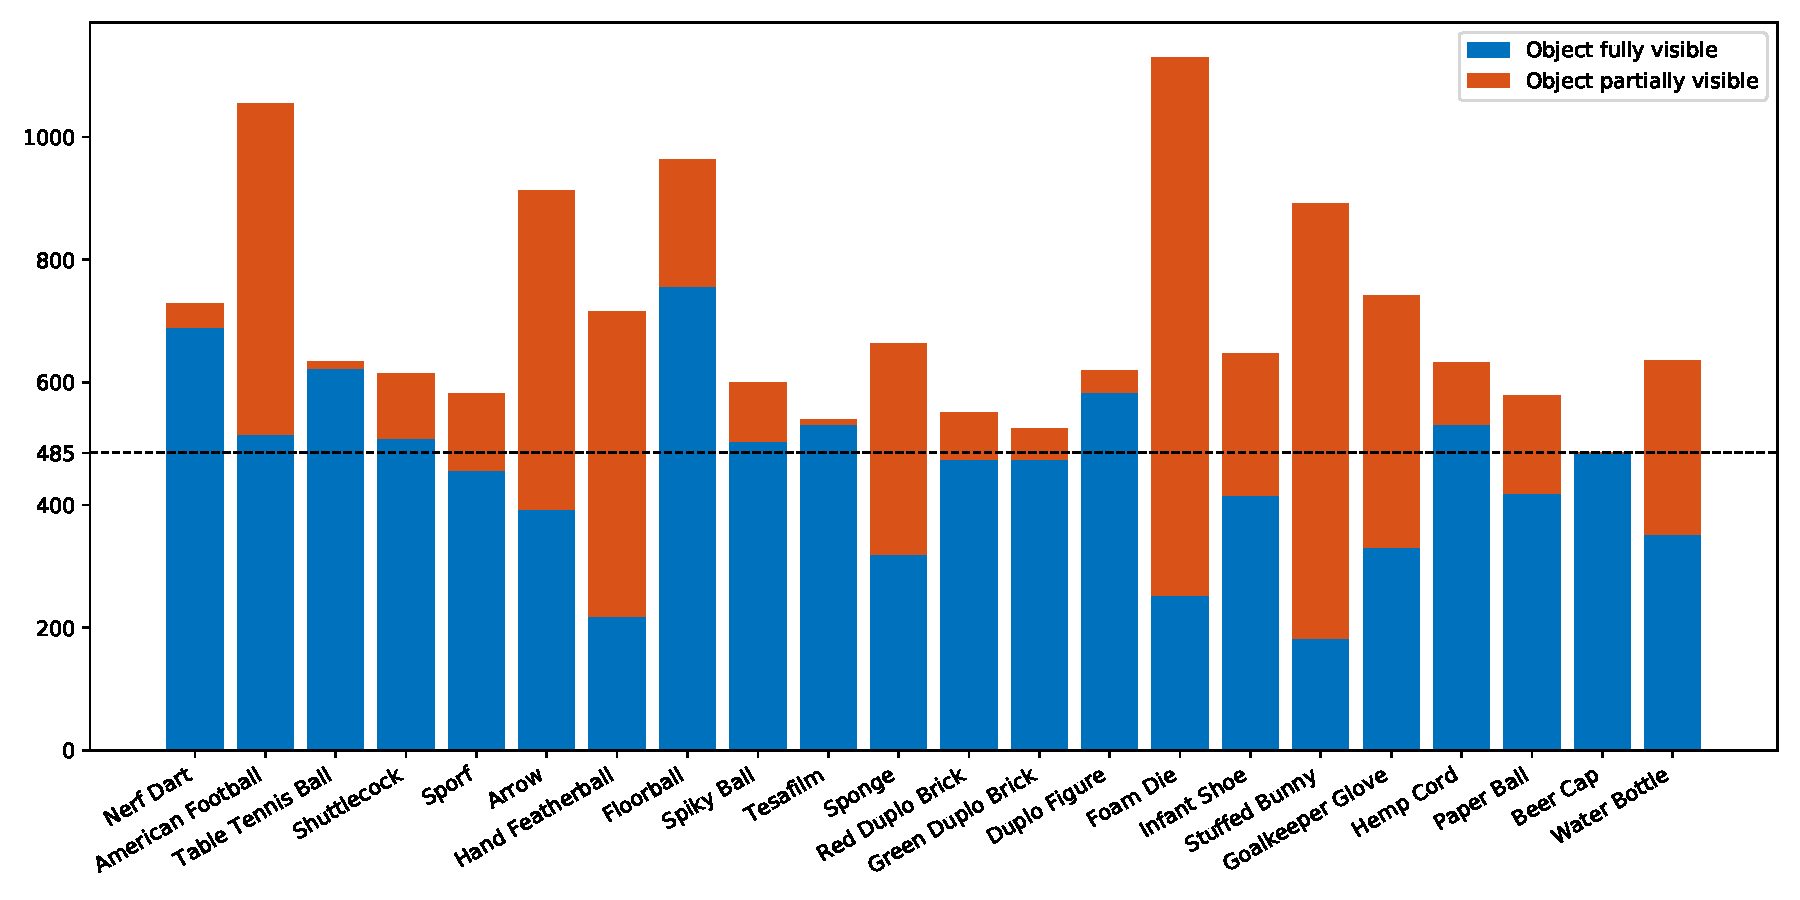
\includegraphics[width=\textwidth]{statistics}
  \caption{Statistics showing the amount of captured frames for each object individually}
  \label{fig:statistics}
\end{figure}





















\subsection{Augmentation}
\label{subsec:training_of_the_cnn:dataset:augmentation}

% There are a few issues with the collected dataset. -> different wording!, specific problems are explained!

% downsampling necessary due to too much data
% The shape of the individual frames is \num{1280}~$\times$~\num{1024}~$\times$~\SI{3}{px} (height, width, number of color channels). % todo: remove the 3 (these are not pixels!)
% The image dimensions of the individual frames are \num{1280}~$\times$~\SI{1024}{px} (width $\times$ height) with three color channels (\acrshort{rgb}).
The image dimensions of the individual frames are $1280\times\SI{1024}{px}$ (width $\times$ height) with three color channels (\acrshort{rgb}).
% This is an enormous amount of input data for a \acrlong{cnn} and would result in an extremely big \acrshort{cnn} model.
% This is an enormous amount of input data for a \acrlong{cnn} and would result in an extremely large amount of trainable parameters.
This is an enormous amount of input data for a \acrlong{cnn} and would result in an extremely large amount of mathematical operations to classify even a single frame.
% This does not only decrease the classification throughput, it also greatly increases the time required to fit the \acrshort{cnn} model. % todo: leave also there or not
% This reduces the classification throughput and thus also greatly increases the required time to fit the \acrshort{cnn} model. % todo: leave also there or not
As a result, the classification throughput is reduced and thus the time required to fit the \acrshort{cnn} model is greatly increased.
% The most important aspect

Another important aspect of the dataset is the fact that it was collected over the course of only two days.
Some objects (e.g. the \textit{Water Bottle}) were even added only on the second day of the data collection. % todo: 'the' before 'Water Bottle'? / % todo: frame or data collection?
% - due to real-world observations (have shown)
Real-world observations have shown that the surrounding ambient light and the orientation of an object have a significant influence on the classification performance.
% - nicht sehr allgemein, bias zu dunkelen umgebungslicht
% During the data colection the ambient light did not change much and therefore
The data collection took place in a relatively dim location and the ambient light did not change much.
% broad spectrum of ambient lights
% - Problem of daylight / flipping
% Therefore, the spectrum of ambient lights is not very broad at all and the classification performance
The classification performance is therefore much better when there is less ambient light.

% Furthermore, the orientation of an object on a frame also influences the classification performance.
Furthermore, the orientation of an object on a frame also impacts the classification performance.
% If, for example, the \textit{Shuttlecock} is deliberately thrown with the plastic feather tail in front of the cork head it could be classified as an entirely diferent object.
% One such problem arises if, for example, the \textit{Shuttlecock} is deliberately thrown with the plastic feather tail in front of the cork head. % todo: maybe feathers, probably not though
One such problem arises if, for example, the \textit{Shuttlecock} is deliberately thrown with the plastic tail feathers in front of the cork head.
% This results in a complete misclassification of the object.
% This would result in a complete misclassification of the object.
Experiments have shown that this results in a complete misclassification of the object.

% maybe use: to counteract (I used to "improve the [...] performance", which is basically the same)
% For those reasons, the individual frames are augmented accordingly.
For those reasons, a range of image data augmentation techniques are used on the individual frames to improve the real-world classification performance \cite{}. % todo: cite https://link.springer.com/content/pdf/10.1186/s40537-019-0197-0.pdf
% todo: Augmentation is done in Python with the use of OpenCV
% The dataset augmentation is done with the Python script \texttt{dataset\_generator.py} and the use of the Python implementation of the \acrfull{opencv}.
% The dataset augmentation is done with the Python script \texttt{dataset\_generator.py}, which uses the Python implementation of the \acrfull{opencv} as well as the NumPy library (provides support for large, multi-dimensional arrays and matrices).
% The dataset augmentation is done with the Python script \texttt{dataset\_generator.py}, which uses the Python implementation of the \acrfull{opencv} as well as the NumPy library.
% The dataset augmentation is done with the Python script \texttt{dataset\_generator.py}, which uses the NumPy library as well as the Python implementation of the \acrfull{opencv}.
The dataset augmentation is done with the Python script \texttt{dataset\_generator.py}, which uses NumPy as well as the Python implementation of the \acrfull{opencv}.
% The dataset augmentation is done with the Python script \texttt{dataset\_generator.py}.
% This script uses the Python implementation of the \acrfull{opencv}, which provides various functions to (e.g. loading and saving images, resizing images, ).
% as well as the NumPy library (provides support for large, multi-dimensional arrays and matrices).
% NumPy provides support for large, multi-dimensional arrays in addition to functions to work on these arrays.
NumPy provides support for large, multi-dimensional arrays and an assortment of functions to work on these arrays \cite{}. % todo: maybe cite https://numpy.org/doc/stable/user/whatisnumpy.html
\acrshort{opencv} provides various image transformation functions (e.g. resizing, color space conversions) and conveniently uses NumPy arrays to represent the images \cite{}. % todo: cite https://docs.opencv.org/3.4.3/d1/dfb/intro.html

% -----------------------
\paragraph{Image Scaling}
% size reduction / Resizing / downsampling / image scaling
% Downsampling
% To reduce the shape of the individual frames, the shape is scaled down
% To reduce the input data of the \acrshort{cnn} model, the individual frames are scaled down by a factor of four in each dimension.
To reduce the input data of the \acrshort{cnn} model, the width and height of the individual frames are each scaled down by a factor of four.
% This results in an image with the dimensions of \num{320}~$\times$~\SI{256}{px} (width $\times$ height) and thus in a data reduction of \num{16}.
This results in an image with the dimensions of $320\times\SI{256}{px}$ (width $\times$ height) and thus in a data reduction of \num{16}.

% size chosen arbitrarily
% good size, important features are still visible
% These dimensions are ideal because the most important features are still visible.
% These dimensions are ideal because the most important features are still visible.
% These dimensions are great because the most important features are still visible.
% These dimensions are great because even the important features of the smallest objects are still visible.
These dimensions are great because even the important features of the smallest objects are still preserved.
% Furthermore, a reasonably deep \acrlong{cnn} should have no problems to diffentiate between the only \num{22} different classes.
Given that the background of the frames remains more or less the same, a reasonably deep \acrshort{cnn} should have no problems distinguishing between the only \num{22} different classes.
% managable with a reasonably deep CNN (smaller than some state-of-the-art CNNs) and a slightly larger input filter
% Furthermore, the
% results in 320 * 256 * 3 = 245760 artificial input neurons (ain) which is managable with a reasonably deep CNN (smaller than some state-of-the-art CNNs)
% The total number of of artificial input neurons of the \acrshort{cnn} model is equal to % this is wrong, this is not a ANN (fully-connected)!
% \[
% \text{Input Neurons} = \text{Width} \cdot \text{Height} \cdot \text{Channels} = 320 \cdot 256 \cdot 3 = \num{245760}.
% \]

The downsampling is achieved with the use of nearest-neighbor interpolation.
% nn more noise/distortion than bilinear and bicubic
% This results in more noise than other interpolation methods, like bilinear or bicubic interpolation.
% This results in more noise and distortion than other interpolation methods, such as bilinear or bicubic interpolation.
This results in more noise and scaling artifacts than other interpolation methods, such as bilinear or bicubic interpolation.
% as well as mosaic and saw tooth phenomenon
% In addition to the noise
% The noise is shown in the form of aliasing
% The distortion is shown in the form of aliasing and 
% The scaling artifacts are shown in figure \ref{fig:augmentation_downsampling} and are the result of aliasing.
The scaling artifacts shown in figure \ref{fig:augmentation_downsampling} are the result of aliasing.
% but simple/fast speed
% The nearest-neighbor interpolation is chosen due to its simplicity and fast execution \cite{}.
The advantages of nearest-neighbor interpolation are its simplicity and fast execution time \cite{}. % todo: cite https://www.atlantis-press.com/proceedings/iccsee-13/4822
% and noise can help against overfitting
Furthermore, the additional noise can improve the generalization and therefore reduce overfitting \cite{}. % todo: cite https://machinelearningmastery.com/train-neural-networks-with-noise-to-reduce-overfitting/

% python implementation with the \acrshort{opencv} function \texttt{cv2.resize}
The Python implementation of the image scaling makes use of the \acrshort{opencv} function \texttt{cv2.resize}.
This function is supplied with three arguments: the NumPy array that represents the image, the desired output image size and the interpolation method \cite{}. % todo: cite https://docs.opencv.org/3.4.3/da/d54/group__imgproc__transform.html#ga47a974309e9102f5f08231edc7e7529d

% Figure \ref{fig:augmentation_downsampling} shows the above mentioned scaling artifacts.
% The above mentioned scaling artifacts are shown in figure \ref{fig:augmentation_downsampling}.

\begin{figure}
  \centering
  \begin{subfigure}[b]{0.45\textwidth}
    \centering
    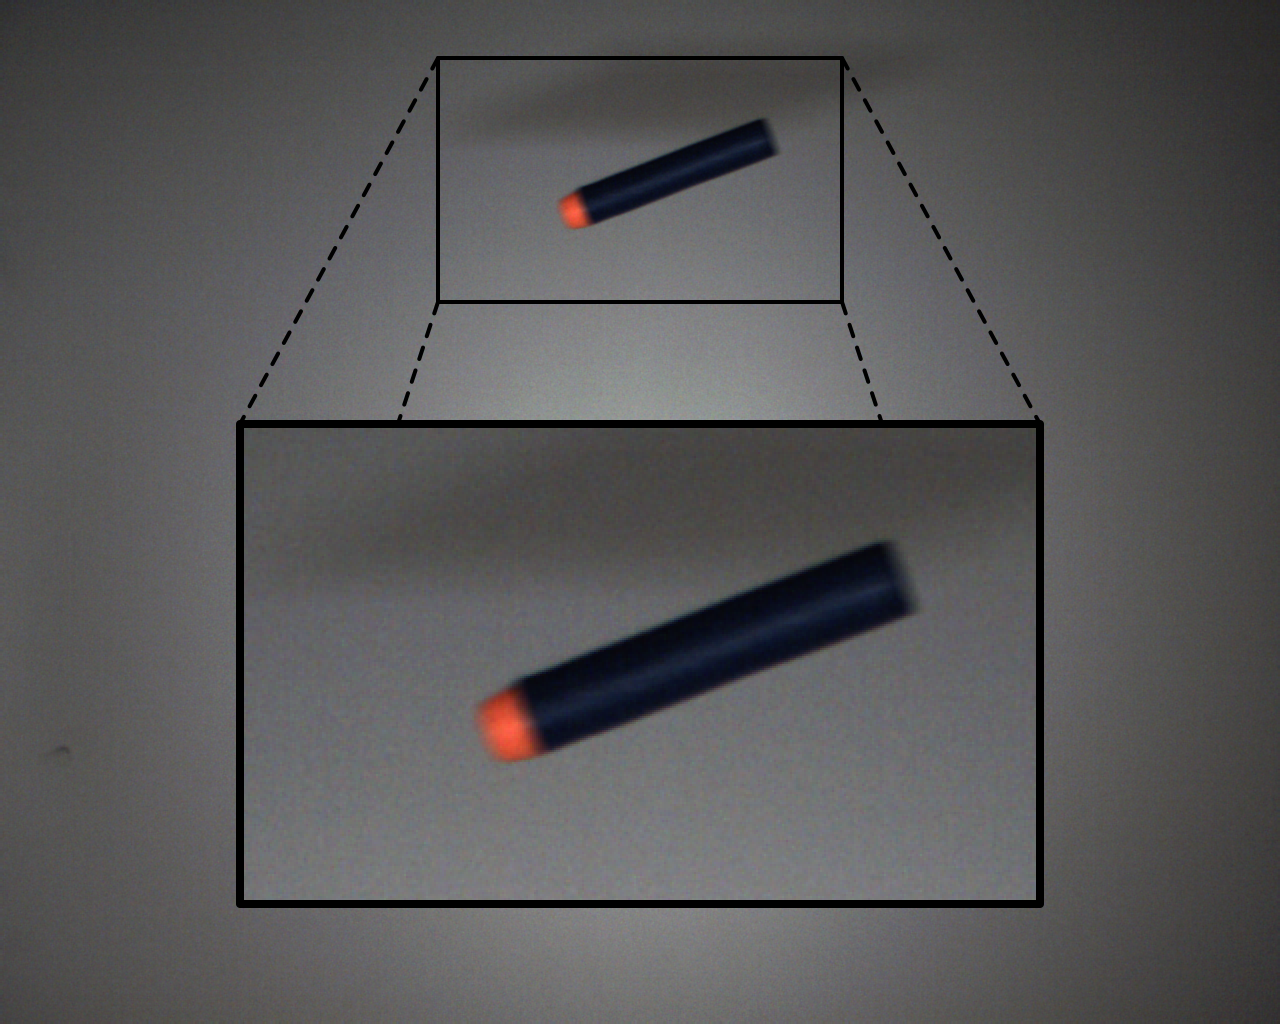
\includegraphics[width=\textwidth]{augmentation_downsampling/1575032863_742_3_nerf-dart_zoom}
    \caption{Original version}
    \label{subfig:ad_original}
  \end{subfigure}
  \begin{subfigure}[b]{0.45\textwidth}
    \centering
    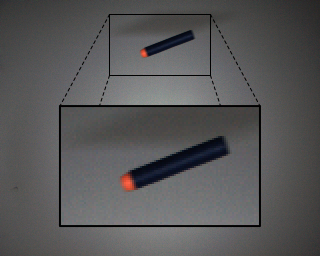
\includegraphics[width=\textwidth]{augmentation_downsampling/1575032863_742_3_nerf-dart_resized_zoom}
    \caption{Scaled-down version}
    \label{subfig:ad_resized}
  \end{subfigure}
  \caption{Example of an original (\subref{subfig:ad_original}) and a scaled-down version (\subref{subfig:ad_resized}) of a frame ($2\times$ inner zoom added to better highlight the difference)}
  \label{fig:augmentation_downsampling}
\end{figure}

% ---------------------
\paragraph{Color Space}
To reduce the dependence on ambient light intensity, the average brightness of the individual frames is changed.
% The rounded average brightness $\overline{B}$ of an image can be calculated using equation \ref{eq:average_brightness}.
The rounded average brightness $B$ of an image can be calculated using equation \ref{eq:rounded_average_brightness}.
% The Python script uses the NumPy function \texttt{np.sum} to compute the sum of all array elements. % todo: put code in appendix?
This equation is implemented in Python with the help of the NumPy function \texttt{np.sum}, which computes the sum of all array elements. % todo: cite https://numpy.org/doc/stable/reference/generated/numpy.sum.html ???
% todo: put code in appendix? If yes, so reference to it: as shown in appendix \ref{app:throw_detection} on line \ref{lst:ln:mean_diff}!

\begin{equation}
  B = \left\lfloor\frac{1}{w\cdot h\cdot c} \cdot \sum\limits_{k=1}^c \sum\limits_{i=1}^h \sum\limits_{j=1}^w \boldsymbol{M}_{ij}^{k} + 0.5\right\rfloor
  \label{eq:rounded_average_brightness}
\end{equation}

where

\begin{tabular}{lll}
  $B$ & = & rounded average brightness \\
  $w$ & = & width of the image \\
  $h$ & = & height of the image \\
  $c$ & = & number of channels \\
  $\boldsymbol{M}^k$ & = & pixel matrix of channel $k$ \\
\end{tabular}
\\

\clearpage % todo: leave this?, probably yes

% The average brightness of the background lies between \num{85} (without ambient light) and \num{160} (with indirect sunlight and artifical ambient light) at various times of the day.
% The average brightness of the background was computed at various times of the day and lies between \num{85} (without ambient light) and \num{160} (with indirect sunlight and artifical ambient light).
The rounded average brightness of the background was computed at various times of the day and lies between \numrange{85}{160}.
% (without ambient light) and (with indirect sunlight and artifical ambient light).
This range includes environments without ambient light as well as environments with indirect sunlight and artifical ambient light.
% steps of 15 were chosen: [85, 100, 115, 130, 145, 160]
In the light of these results, a step size of \num{15} was chosen to cover this spectrum of ambient light intensities.
This results in the following six discrete average brightness levels: \num{85}, \num{100}, \num{115}, \num{130}, \num{145} and \num{160}.

% Since the collected frames contain objects, only the first frame of a throw (which presumably consists of mostly background) is used to evaluate the average brightness durinng that throw
% Calculating the average brightness of the individual frames is problematic, as the frames do not only consist of background but also have objects on them.
Calculating the average brightness of the individual frames is problematic, as the frames contain objects in addition to the background. % todo: maybe use display or show
% For this reason, only the first frame of a throw (which presumably consists mainly of background) is used to evaluate the average brightness durinng that throw.
% For this reason, only the first frame of a throw (which presumably consists mainly of background) is used to evaluate the average brightness of the entire throw.
% For this reason, only the first frame of a throw (which presumably consists mainly of background) is used to compute the average brightness for all frames of that throw.
For this reason, only the first frame of a throw (which presumably consists mainly of background) is used to compute the average brightness $B_1$.
% after that the brightness augmentation / adaption is performed on all frames of the throw according to the average brightness of the first frame of that throw
% This value is then used to adjust the brightness of all frames of that throw.
This value is then used to determine the required brightness offset $\Delta$ for all frames of that throw as shown in equation \ref{eq:offset_calculation}. % todo: use "this throw"?

\begin{equation}
  \Delta = B_{\text{des}} - B_1
  \label{eq:offset_calculation}
\end{equation}

where

\begin{tabular}{lll}
  $\Delta$ & = & required brightness offset \\
  $B_{\text{des}}$ & = & desired, rounded average brightness \\
  $B_1$ & = & rounded average brightness of the first frame of the throw \\
\end{tabular}
\\

% talk about how the adjustment is done (by computen the required brightness offset and then adding the offset to each pixel of each channel individually)
% mention that there are no overflow but clipping is happening
% talk about uint8!
The brightness adjustment is done according to equation \ref{eq:brightness_adjustment}.
% The Python implementation requires two steps to implement
% The equation is implemented in two steps
The implementation of this equation in Python consists of two steps.
In a first step, the required brightness offset $\Delta$ is added to each pixel of each color channel individually.
% The pixel values are unsigned integers in the range between \num{0}--\num{255}.
% These unsigned integers must be in the range between \num{0}--\num{255} (\SI{8}{bit}).
% The pixel values are unsigned integers, which must be in the range between \num{0} and \num{255} (\SI{8}{bit}).
The pixel values are 8-bit unsigned integers, which must be in the range between \numrange{0}{255}.
% To ensure this range is not exceeded, the values are clipped with the NumPy function \texttt{np.clip}.
% To ensure this range is not exceeded, the values are clipped in a second step.
% These values are clipped in a second step, to ensure that the range is not exceeded.
In order to ensure that this range is not exceeded, the values are clipped in a second step.
For this purpose, the NumPy function \texttt{np.clip} is used \cite{}. % todo: cite https://numpy.org/doc/stable/reference/generated/numpy.clip.html
% todo: if code is added in the appendix, reference to it (and also to the specific line)

\begin{equation}
  % \boldsymbol{A}_{ij}^{k} = \min\!\left(0,\:\max\!\left(255,\:\boldsymbol{M}_{ij}^{k} + o\right)\right), % old alternative
  A_{i,j}^{k} =
  \begin{cases}
    0 & M_{i,j}^{k} + \Delta < 0 \\
    M_{i,j}^{k} + \Delta & 0\leq M_{i,j}^{k} + \Delta\leq 255 \\
    255 & M_{i,j}^{k} + \Delta > 255 \\
  \end{cases}
  \label{eq:brightness_adjustment}
\end{equation}

where

\[
  % 1\leq i\leq h \quad \text{and} \quad 1\leq j\leq w \quad \text{and} \quad 1\leq k\leq c
  i = 1, 2, \dots, h \quad \text{and} \quad j = 1, 2, \dots, w \quad \text{and} \quad k = 1, 2, \dots, c
\]

and

\begin{tabular}{lll}
  $A_{i,j}^{k}$ & = & element $i,j$ of the $k$-th channel augmented pixel matrix $\boldsymbol{A}$ \\
  $M_{i,j}^{k}$ & = & element $i,j$ of the $k$-th channel pixel matrix $\boldsymbol{M}$ \\
  $\Delta$ & = & required brightness offset \\
  $h$ & = & height of the image \\
  $w$ & = & width of the image \\
  $c$ & = & number of channels \\
\end{tabular}
\\

% figure of brightnesses: original, 85 - 160
% explain the example!
% Figure \ref{fig:augmentation_brightness} shows examples of resized frames of the \textit{Water Bottle}, where the brightness was adjusted according to the desired brightness levels.
% Figure \ref{fig:augmentation_brightness} shows an example of the resized frames of the \textit{Water Bottle}, where the brightness was adjusted according to the desired brightness levels.
Figure \ref{fig:augmentation_brightness} shows an example of the resized frames of the \textit{Water Bottle}, where the brightness levels were adjusted.
For this example, frame \num{12} of throw \num{575} was used.
% The rounded average brightness of the first frame of this throw $B_1$ is equal to \num{101}, whereas $B_{12}$ of frame \num{12} is equal to \num{99}.
The rounded average brightness of the first frame of this throw $B_1$ is equal to \num{101}, whereas $B_{12}$ is equal to \num{99}.
% Therefore, a difference of \num{-2} in regards to the desired brightness levels is expected.
% Therefore, an additional offset of \num{-2} is expected in regard to the desired brightness levels.
Therefore, an additional offset of \num{-2} in regard to the desired brightness levels is expected.
This is due to the fact that the required brightness offset is determined by using the rounded average brightness of the first frame rather than the frame that is being adjusted. % todo: is this sentence too much?

\begin{figure}
  \centering
  \begin{subfigure}[b]{0.15\textwidth}
    \centering
    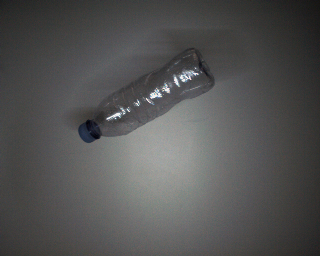
\includegraphics[width=\textwidth]{augmentation_brightness/1575026107_575_12_water-bottle_85}
    \caption{$B = 83$}
    \label{subfig:ab_85}
  \end{subfigure}
  \begin{subfigure}[b]{0.15\textwidth}
    \centering
    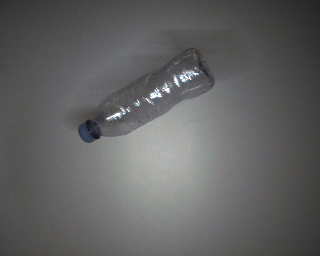
\includegraphics[width=\textwidth]{augmentation_brightness/1575026107_575_12_water-bottle_100}
    \caption{$B = 98$}
    \label{subfig:ab_100}
  \end{subfigure}
  \begin{subfigure}[b]{0.15\textwidth}
    \centering
    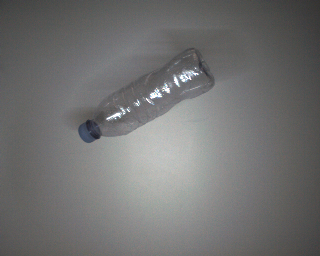
\includegraphics[width=\textwidth]{augmentation_brightness/1575026107_575_12_water-bottle_115}
    \caption{$B = 113$}
    \label{subfig:ab_115}
  \end{subfigure}
  \begin{subfigure}[b]{0.15\textwidth}
    \centering
    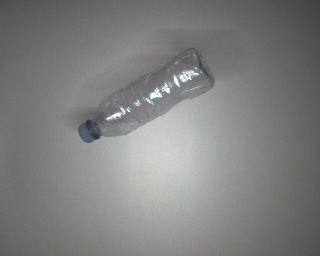
\includegraphics[width=\textwidth]{augmentation_brightness/1575026107_575_12_water-bottle_130}
    \caption{$B = 128$}
    \label{subfig:ab_130}
  \end{subfigure}
  \begin{subfigure}[b]{0.15\textwidth}
    \centering
    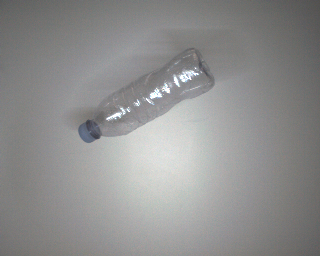
\includegraphics[width=\textwidth]{augmentation_brightness/1575026107_575_12_water-bottle_145}
    \caption{$B = 143$}
    \label{subfig:ab_145}
  \end{subfigure}
  \begin{subfigure}[b]{0.15\textwidth}
    \centering
    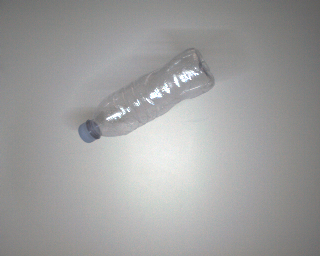
\includegraphics[width=\textwidth]{augmentation_brightness/1575026107_575_12_water-bottle_160}
    \caption{$B = 158$}
    \label{subfig:ab_160}
  \end{subfigure}
  \caption{Examples of resized frames of the \textit{Water Bottle}, where the brightness was adjusted according to the desired brightness levels}
  \label{fig:augmentation_brightness}
\end{figure}

% ------------------
\paragraph{Flipping}
% To improve the orientation-independence of the objects, each frame is flipped vertically and horizontally.
Each frame is flipped vertically and horizontally to improve the orientation-independence of the objects in the frames.
% This also decreases the influence of the shadow that the object casts.
% Furthermore, the influence of the shadow that the object casts is decreased, which supports the generalization.
Furthermore, the influence of the shadow that the object casts is decreased.
An example of these reflections is shown in figure \ref{fig:augmentation_flipping}.

The Python implementation uses the \acrshort{opencv} function \texttt{cv2.flip} to flip the frames around the x-axis (vertically) and around the y-axis (horizontally) \cite{}. % todo: cite https://docs.opencv.org/3.4.3/d2/de8/group__core__array.html#gaca7be533e3dac7feb70fc60635adf441
% todo: if the code is added in the appendix, reference to it

% figure of flipping (shuttlecock): original, vertical, horizontal
\begin{figure}
  \centering
  \begin{subfigure}[b]{0.3\textwidth}
    \centering
    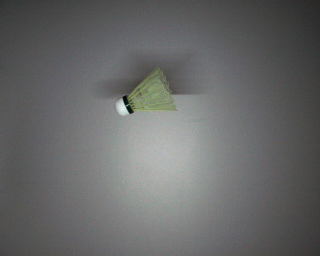
\includegraphics[width=\textwidth]{augmentation_flipping/1575023302_468_9_shuttlecock}
    \caption{Unaugmented}
    \label{subfig:af_resized}
  \end{subfigure}
  \begin{subfigure}[b]{0.3\textwidth}
    \centering
    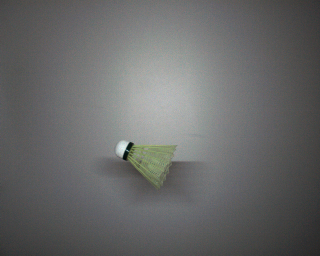
\includegraphics[width=\textwidth]{augmentation_flipping/1575023302_468_9_shuttlecock_v}
    \caption{Vertically flipped}
    \label{subfig:af_vertical}
  \end{subfigure}
  \begin{subfigure}[b]{0.3\textwidth}
    \centering
    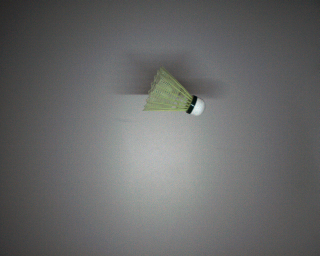
\includegraphics[width=\textwidth]{augmentation_flipping/1575023302_468_9_shuttlecock_h}
    \caption{Horizontally flipped}
    \label{subfig:af_horizontal}
  \end{subfigure}
  \caption{Example of a resized frame of the \textit{Shuttlecock} (\subref{subfig:af_resized}), which was flipped vertically (\subref{subfig:af_vertical}) and horizontally (\subref{subfig:af_horizontal})}
  \label{fig:augmentation_flipping}
\end{figure}










\subsection{Splitting}
\label{subsec:training_of_the_cnn:dataset:splitting}
% During the training of the 
% The fitting and verification process of the \acrshort{CNN} model requires three splits of the dataset.
% During the fitting and verification process of the \acrshort{cnn} model, three splits of the dataset are required.
During the fitting and evaluation process of the \acrshort{cnn} model, three splits of the dataset are required.
% requires several splits
% The various splits and their respective use is summarized in table \ref{tab:dataset_splits}.
These required splits and their respective use is summarized in table \ref{tab:dataset_splits}.

% splits:
% training dataset (~70%): used to fit the model
% validation dataset (~15%): unbiased evaluation of the model fit on the training dataset while tuning model hyperparameters
% test dataset (~15%): unbiased evaluation of the final model fit on the training dataset
% calibration dataset (45 x 22 = 990 images): small unlabeled dataset for calibration (during the quantization) taken from the validation dataset [5..45 frames per class (110..990)]
\begin{table}
  \caption{Overview of the required dataset splits \cite{}} % todo: cite https://machinelearningmastery.com/difference-test-validation-datasets/
  \label{tab:dataset_splits}
  \centering
  \begin{tabular}{llp{10cm}}
    \toprule
    \textbf{Dataset} & \textbf{Split} & \textbf{Description} \\
    \midrule
    \textbf{Training} & \SI{70}{\percent} & The training split is used to fit the model. \\
    \midrule
    % \textbf{Validation} & \SI{15}{\percent} & The validation split provides an unbiased evaluation of a model fit while tuning hyperparameters of the model. \\
    \textbf{Validation} & \SI{15}{\percent} & The validation split provides an evaluation of a model fit while tuning hyperparameters of the model. \\
    \midrule
    \textbf{Test} & \SI{15}{\percent} & The test split provides an unbiased evaluation of the final model fit (used to compare fit with other final models). \\
    \bottomrule
  \end{tabular}
\end{table}

% talk about not reusing images! (I think the word split implies this)
% Some important 
It is crucial that the dataset splits are used in the right way.
% It is important that validation and the test datasets are never used for the actual training.
% It is important that the validation and the test splits are never used for the actual training.
% It is important that the validation and the test splits are never used to fit the model.
For example, the validation and the test splits must never be used to fit the model.
% Furthermore, only the validation dataset must be used to tune hyperparameters.
% The evaluation with the validation split becomes more biased as the classification performance is increased by tuning the hyperparameters of the model.
% Another important aspect is that, the evaluation with the validation split becomes more biased as the classification performance is increased by tuning the hyperparameters of the model.
Furthermore, it is important to know that the evaluation with the validation split becomes more biased as the classification performance is increased by tuning the hyperparameters of the model.
For this reason, a test split is used to evaluate and compare the final model fit.

% \textbf{Calibration} & \num{990} & small unlabeled dataset used for calibration during the quantization process \\
% (taken from the validation dataset [5..45 frames per class (110..990)])
The quantization process requires a small unlabeled dataset consisting of \numrange{100}{1000} frames for the calibration of the quantized model.
% The unlabeled calibration dataset consists of frames from the validation dataset.
% Seeing that the calibration of the quantized model has great similarities to tuning hyperparameters, the required frames are chosen at random from the validation split.
% Seeing that the calibration of the quantized model bears many similarities to tuning hyperparameters, the required frames are chosen at random from the validation split.
Seeing that the calibration of the quantized model has many similarities to the tuning of the hyperparameters, the required frames are chosen at random from the validation split.
% Seeing that the calibration of the quantized model has many similarities to the tuning of the hyperparameters, \num{990} frames (a multiple of the \num{22} classes) are chosen at random from the validation split.
In total, \num{990} frames are chosen from the validation split (largest possible multiple of the \num{22} classes).
% \num{990} frames are chosen at random from the validation split.
% In this case, the calibration dataset is a subset of the validation dataset without labels.
The calibration dataset is thus a subset of the validation dataset without labels.

% ------------------------
\paragraph{Implementation}
% Python implementation
% dataset_generator.py to fix the problem => probably individually for augmentation and splitting
The splitting of the dataset is implemented in the Python script \texttt{dataset\_generator.py}, which uses NumPy, \acrshort{opencv} and the standard library.

% database is used to gather all the necessary information about the dataset
% use of the database (MySQL), explain the different fields
In a first step, the necessary information about the dataset is fetched from the \acrshort{mysql} database, which is used to store the labels, the file names and other useful metadata.
Table \ref{tab:tab_frames_structure} lists all columns of the database table \texttt{aionfpga.frames}.

\begin{table}
  \caption{Structure of the \acrshort{mysql} database table \texttt{aionfpga.frames}}
  \label{tab:tab_frames_structure}
  \centering
  \begin{tabular}{llll}
    \toprule
    \textbf{Column} & \textbf{Type} & \textbf{Length} & \textbf{Description} \\
    \midrule
    id & \texttt{INT} &  & Sequence number (unique identifier) \\
    timestamp & \texttt{INT} &  & The Unix timestamp at the time of the throw \\
    throwid & \texttt{INT} &  & Throw sequence number \\
    frameid & \texttt{INT} &  & Frame sequence number within a throw \\
    frame & \texttt{VARCHAR} & 255 & The file name of the frame \\
    object & \texttt{VARCHAR} & 255 & The name of the object in the frame (label) \\
    framegood & \texttt{INT} &  & \texttt{0}: frame unusable | \texttt{1}: frame usable \\
    partial & \texttt{INT} &  & \texttt{0}: object fully visible | \texttt{1}: object partially visible \\
    \bottomrule
  \end{tabular}
\end{table}

% use under-sampling of the dataset
% uses only ~66.6% of the entire frames
% To balance the dataset 
% To ensure the dataset is balanced
% The first step is to balance the slightly imbalanced dataset.
% A first step ensures that the slightly imbalanced dataset 
% A first step takes care of the slightly imbalanced dataset.
% In a first step, the slight imbalance in the dataset is mitigated.
The slight imbalance in the dataset is mitigated in a next step.
There are several different methods to ensure that the dataset is balanced (e.g. collecting more data, resampling).
For the sake of simplicity, undersampling is used to remove samples from the overrepresented classes \cite{}. % todo: cite https://machinelearningmastery.com/tactics-to-combat-imbalanced-classes-in-your-machine-learning-dataset/

% randomization of the balancing
% Only the amount of frames in the minority class is used from all classes.
% Among all classes, only the number of images in the minority class is used.
% The actual implementation randomly chooses the amount of frames in the minority class from each class.
The actual implementation randomly selects frames from each class. % todo: use picks?
The number of selected frames is equal to the number of frames in the minority class.
% is ordered, the required samples are chosen at random.
% To ensure that each split 
% The pseudorandom function used for the selection process is seeded to ensure consistent results during tests.
The pseudorandom function used for the selection process is seeded to ensure repeatable results during different tests.
In this case, this results in a loss of about \SI{30.9}{\percent} of the collected frames.

% augmentation is perfomred according to section ...
In a third step, the data augmentation discussed in section \ref{subsec:training_of_the_cnn:dataset:augmentation} is performed.
% Since the original frames are preserved as well, the size of the dataset increases by a factor of seven. % brightness
% Since the original frames are preserved as well, the size of the dataset increases by a factor of three. % flipping
The frames are first resized, then their brightness is adjusted and lastly they are flipped.
% An important fact is that the original (unaugmented) frames are preserved as well.
The brightness adjustment increases the size of the dataset by a factor of seven and the flipping by a factor of three.
% This is due to the fact, that the original frames are preserved as well and results in a total dataset increase of \num{21}.
This is due to the fact, that the original frames are preserved as well and results in a total increase of the dataset size by a factor of \num{21}.
% Due to the fact, that the original frames are preserved as well  results in a total dataset increase of \num{21}.
Original refers in this case to the resized frames.

% randomization of all augmented frames (split is done here)
The next step is the actual splitting of the dataset.
For this purpose, the entire dataset is shuffled and then split according to table \ref{tab:dataset_splits}.

% format how the dataset is saved (numpy arrays [.npy])
% In a last step, the dataset splits are saved to the disk.
% The frames and the labels are stored separately.
In a last step, the frames and the labels of the dataset splits are separately saved to the disk.
% they have to be saved in batches because the size would be too big to be load into memory (maybe talk about float32)
% save_batches function!
% Due to the sheer number of frames in the dataset splits, the actual implementation saves the frames in batches of \num{32}.
Due to the sheer number of frames in the dataset splits, the frames are saved in batches of \num{32}.
% For this reason, \num{32} frames at a time are stored in a four-dimensional NumPy array with the shape of 32 $\times$ 256 $\times$ 320 $\times$ 3 (batch size $\times$ height $\times$ width $\times$ number of color channels) of type \texttt{np.uint8}.
% For this reason, \num{32} frames at a time are stored in a four-dimensional NumPy array of type \texttt{np.uint8} with a shape of 32~$\times$~256~$\times$~320~$\times$~3 (batch size $\times$ height $\times$ width $\times$ number of color channels).
For this reason, \num{32} frames at a time are stored in a four-dimensional NumPy array of type \texttt{np.uint8} with a shape of $32\times 256\times 320\times 3$ (batch size $\times$ height $\times$ width $\times$ number of color channels).
% also format of the labels (number from 0-21)
The \num{22} different labels of the classes (object names) are mapped to a unique number between \num{0} and \num{21}.
This allows for an efficient way to store the labels in one-dimensional NumPy arrays of type \texttt{np.uint8}.
% This array 
The length of these label arrays is determined by the number of frames in the respective splits.
% The labels are stored in the same order as the frames.
% The labels are then 

% For each split, both the batch arrays and the label array are saved ...
For each split, both the batch arrays and the label array are saved to the disk in the binary NumPy (\texttt{.npy}) file format \cite{}. % todo: cite https://numpy.org/doc/stable/reference/generated/numpy.lib.format.html#module-numpy.lib.format
% This is done using NumPy ... in the binary \texttt{.npy} format.
% This array is then saved to the disk in the binary NumPy (\texttt{.npy}) file format.
This allows for fast loading of the dataset from the disk \cite{}. % todo: cite https://towardsdatascience.com/why-you-should-start-using-npy-file-more-often-df2a13cc0161

% This is implemented in the function \texttt{save\_batches}.
% This last step is implemented in the function \texttt{save\_batches} (see listing \ref{lst:save_batches}).
Listing \ref{lst:save_batches} shows the function \texttt{save\_batches}, which implements this last step.

\begin{lstlisting}[style=python, caption={Python function \texttt{save\_batches} to save the batch arrays and the label array}, label=lst:save_batches]
def save_batches(frames_name, labels_name, dst, frame_names, batch_size):

  num_frames = len(frame_names)
  num_batches = math.ceil(num_frames / batch_size)

  labels = np.empty((num_frames,), dtype=np.uint8)
  for idx in range(num_batches):
    start = idx * batch_size
    end = start + batch_size
    frame_names_slice = frame_names[start:end]

    frames = np.empty((len(frame_names_slice),) + fh.inf_shape, dtype=np.uint8)
    for i, frame in enumerate(frame_names_slice):
      obj_san = frame.split('_')[3]
      label = fh.objects_san.index(obj_san)
      frames[i] = cv2.imread(str(fh.dir_frames_augmented / f'{frame}.png'))
      labels[idx * batch_size + i] = label

    np.save(dst / f'{frames_name}_batch_{idx}_of_{num_batches}.npy', frames)

  np.save(dst / f'{labels_name}.npy', labels)
\end{lstlisting}

% ----------------
\paragraph{Result}
% Information about the final dataset!
% list the total amount of frames for each split
% talk about the total size
% \SI{7.69}{GiB} (each one of val and test) 33594 frames
The toal number of frames after the augmentation is equal to \num{224070}.
The final training dataset consists of \num{156882} frames and requires \SI{35.91}{GiB} of disk space.
The validation and test datasets each comprise of \num{33594} frames and require \SI{15.38}{GiB} of disk space together.
% todo: too much 'the'




